% -*- coding: utf-8 -*-
\chapter{時間・空間制限下のヒューリスティック探索}
\label{ch:heuristic-search-variants}


A*探索などのヒューリスティック探索は時間と空間の両方がボトルネックとなりうる。
すなわち、A*はノードを一つずつ展開していかなければならないので、その数だけノード展開関数を実行しなければならない。また、A*は重複検出のために展開済みノードをすべてクローズドリストに保存する。なので、必要な空間も展開ノード数に応じて増えていく。

残念ながら、ほぼ正しいコストを返すヒューリスティック関数を使っても、A*が展開するノードの数は指数的に増加することが知られている\cite{helmert:08}。

そのため、ヒューリスティックの改善のみならず、アルゴリズム自体の工夫をしなければならない。
この章では時間・空間制約がある場合のA*の代わりとなるヒューリスティック探索の発展を紹介する。
これらのアルゴリズムはメリット・デメリットがあり、問題・計算機環境によって有効な手法が異なる。よって、A*を完全に取って代わるものは一つもないと言える。

\define{ビームサーチ}{beam-search}{ビームサーチ}は非最適解を高速に見つけるための手法である。実行時間・メモリ消費の双方が限られた状況においてなるべく良い解を見つけたい場合に使われる。自然言語処理などでも使われている。
\define{分枝限定法}{branch-and-bound}{ぶんしげんていほう}は非最適解を見つけやすい問題で特に有効な手法であり、メモリ消費が小さいというメリットがある。
\define{反復深化A*}{iterative deepening A*}{はんぷくしんかエースター}は線形メモリアルゴリズムであり、メモリが足りない問題で使われる。
\define{両方向探索}{bidirectional search}{りょうほうこうたんさく}は初期状態とゴール状態の両方から探索をはじめ、二方向の探索が交わるところを探す方法である。ヒューリスティック関数の精度が悪いときに有用である場合が多いことが知られている。
\define{シンボリック探索}{symbolic search}{シンボリックたんさく}は\define{二分決定グラフ}{Binary Decision Diagram}{にぶんけっていぐらふ}を用いて状態集合を表すことによってノードの集合に対して一度に演算を行う手法である。
新奇性に基づく枝刈りは目新しくない状態は枝刈りする。
% 外部メモリ探索は状態空間がメモリに収まりきらない問題に対して外部記憶を使うことで解決する手法である。
\define{並列探索}{parallel search}{へいれつたんさく}は複数のコアや計算機を使うことでメモリと計算時間の両方の問題を解決する。

\section{ビームサーチ (Beam Search)}
\label{sec:beam-search}

\define{ビームサーチ}{beam-search}{ビームサーチ}は実行時間・メモリ消費の双方が限られた状況においてなるべく良い解を見つけたい場合に使われる。
実装は非常にシンプルである。探索中にオープンリストがビーム幅よりも大きくなった場合、最も有望ではないノードを取り除いていくというものである。
プライオリティ関数を$g$とする場合、すなわち幅優先探索とする場合を特にビームサーチと呼ぶ場合もある。
ビームサーチは許容的ではない。有望ではないノードを探索から取り除いているため、最適解を発見する保証がない。
ビームサーチのメリットはメモリ効率である。オープンリストの大きさを一定に保つため、メモリの消費量が抑えられる。
より正確にはビームサーチのメモリ消費量はビーム幅と探索の深さの積に比例する ($O(kd)$)。
特に重複検出を必要としないような問題であればクローズドリストも取り除くことでメモリ消費量を探索ノード数に関わらず一定にすることができる。
メモリにハード制約があるような状況下であるときに有効である。
ビームサーチはビーム幅を適切に設定することが良い解を発見するために重要である。
ビーム幅を動的に設定する方法はいくつか提案されている \cite{lemons2022beam}。


\begin{algorithm}
	\caption{ビームサーチ (Beam Search)}
	\label{alg:beam-search}
		\Input{非明示的状態空間グラフ $(s, Goal, Expand, w)$、プライオリティ関数 $f$、ビーム幅 $k$}
		\Output{$s$からゴール状態への経路、経路が存在しなければ$\emptyset$}
		$Open \leftarrow \{s\}$, $Closed \leftarrow \{s\}$, $d(s) \leftarrow 0$, $g(s) \leftarrow 0$\;
		\While{$Open \neq \emptyset$} {
					$u \leftarrow \argmin_{u' \in Open} f(u')$ \;
			$Open \leftarrow Open \setminus \{u\} $\;

			\While {$|Open| > k$} {
				$u \leftarrow \argmax_{u' \in Open} f(u')$
				$Open \leftarrow Open \setminus \{u\}$\;
			}

			\If {$Goal(u)$} {
				\Return $Path(u)$\;
			}
			\For {each $v \in Expand(u)$} {
			  \If{$v \notin Closed$ {\bf or} $g(u) + w(u, v) < g(v)$} {
						$Open \leftarrow Open \cup \{v\}$\;
				$d(v) \leftarrow d(u) + 1$\;
				$g(v) \leftarrow g(u) + w(u, v)$\;
						$parent(v) \leftarrow u$\;
					  }
			  \If{$v \notin Closed$} {
						$Closed \leftarrow Closed \cup \{v\}$\;
					  }
			}
		 }
		\Return $\emptyset$\;
\end{algorithm}


\section{分枝限定法 (Branch-and-Bound)}
\label{sec:branch-and-bound}

\define{分枝限定法}{branch-and-bound}{ぶんしげんていほう}は非最適解が簡単に見つけられるが最適解を発見するのは難しい問題、例えば巡回セールスパーソン問題のような問題に使われることが多い。
分枝限定法は広くコンピュータサイエンスで使われる汎用的な考え方である。
アイディアとしては問題を複数のサブ問題に分割(branch)し、これまでに得られた解よりも悪い解しか得られないサブ問題を枝刈りする(bound)、というアイディアである。
特にメモリ効率の良い深さ優先分枝限定法 (Depth-First Branch-and-Bound)が探索分野ではよく使われる。
分枝限定法の処理は一般的な木探索に加えて枝刈りが行う (アルゴリズム \ref{alg:branch-and-bound})。

% TODO
\begin{algorithm}
\caption{深さ優先分枝限定法 (Branch-and-Bound)}
\label{alg:branch-and-bound}
        \Input{非明示的状態空間グラフ $(\mathcal{E}, u_0, \mathcal{G}, w)$、ヒューリスティック関数 $h$}
	\Output{$u_0$からゴール状態への経路、経路が存在しなければ$\emptyset$}
	$U \leftarrow \infty$\;
	$P \leftarrow \emptyset$\;
	$(U, P) \leftarrow DFB\&B((\mathcal{E}, u_0, \mathcal{G}, w), 0, U, P)$\;
	\Return $P$\;
\end{algorithm}

\begin{algorithm}
\caption{DFB\&B$((\mathcal{E}, u, \mathcal{G}, w), g, U, P)$: 分枝限定法の再帰計算}
\label{alg:branch-and-bound-rec}
	\If {$\mathcal{G}(u)$} {
		\If {$g < U$} {
			$U \leftarrow g$\;
			$P \leftarrow Path(u)$\;
		}
	}
  \Else {
    $Succ(u) \leftarrow \mathcal{E}(u)$, sorted according to $h$\;
	  \For {$v \in Succ(u)$} {
	    \If {$g + h(v) < U$} {
	      $(U, P) \leftarrow DFB\&B((\mathcal{E}, v, \mathcal{G}, w), g + w(u, v), U, P)$\;
	    }
	  }
  }
  \Return $(U, P)$
\end{algorithm}

一般に、アルゴリズムの実行に従って最適解とは限らない解を次々と発見する手法において分枝限定法の考え方が採用できる。すなわち現在発見された中でもっとも良い解(incumbent solution)を用いて探索範囲を限定していくアイディアである。
A*探索と比較して分枝限定法の利点は、\define{任意時間アルゴリズム}{anytime algorithm}{にんいじかんアルゴリズム}であることである。
任意時間アルゴリズムとはプログラムを適当なタイミングで停止しても解を返すアルゴリズムを指す。
A*探索は最適解を発見するまで他の非最適解を発見することはない。一方、分枝限定法はすぐに何かしらの解を見つけることができる。そして探索の過程で現在の解よりも良い解を発見し、だんだんと解のクオリティを上げていき、最終的に最適解を発見する。
そのため、どのくらい長い間探索に時間をかけてよいかが分からない場合、任意時間アルゴリズムは理想的である。
関連して、A*のそのような問題を解決した\define{任意時間A*}{Anytime A*}{にんいじかんエースター}というアルゴリズムもある \cite{likhachev2004ara,hansen2007anytime,richter2010joy}。例えば単純にwA*において$w$の値を大きなものからだんだんと1に近づける方法がシンプルで効率的である。
A*や任意時間A*と比較した分枝限定法のもう一つの利点はオープンリストなどのデータ構造を必要としない深さ優先探索であることである。そのためメモリ・キャッシュ効率が良い。一方、重複検出を行わない木探索であるため、ノードの重複が多いドメインでは性能が悪いことが多い。


\section{反復深化深さ優先探索 (Depth First Iterative Deepening)}
\label{sec:depth-first-iterative-deepening}
A*探索は時間・空間の両方がボトルネックになるが、現代の計算機環境では多くの場合空間制約がよりネックになる。
これはA*が重複検出のために展開済みノードをすべてクローズドリストに保存していることに起因する。

\ref{sec:graph-search-algorithm}節で述べたように、重複検出は正しい解を返すためには必須ではない。グラフに対して木探索を行うことも出来る。
しかしながら、単純な幅優先木探索・深さ優先木探索はパフォーマンスの問題がある。

\define{反復深化深さ優先}{depth first iterative deepening}{はんぷくしんかふかさゆうせん} (DFID)は深さ優先探索もメモリ効率と幅優先探索の効率性を併せ持った賢いアルゴリズムである \cite{korf:85a,russelln03}。
アイディアとしては、閾値$cost$を1ずつ大きくしながら、繰り返しコスト制限付き深さ優先 (CLDFS)を実行する (アルゴリズム\ref{alg:depth-first-iterative-deepening})。CLDFSが解を見つければその解を返して停止し、見つけられなければ$cost$を1つ大きくしてもう一度CLDFSを実行する。

DFIDは閾値を大きくする度に一つ前のイテレーションで展開・生成したノードをすべて展開・生成しなおさなければならない。各イテレーション内でもクローズドリストを保持していないために重複検出が出来ない。なので、アルゴリズム全体を通して大量の重複ノードが出る可能性がある。
一見非常に効率が悪いように思えるかもしれないが、実はあまり損をしないことが多い。分枝数を$b$、最適解のコストを$c^*$とする。DFIDは$c^*$回目のイテレーションで生成するノードの数はおおよそ$1 + b + b^2 + ... + b^{c^*} = O(b^{c^*})$である。$c^* - 1$回目のイテレーションで生成されるノードの数はその数のおよそ$1 / b$倍である。$c^* - 2$回目のイテレーションではその更に$1 / b$倍と、指数的に生成ノード数は減っていく。そのため、DFID全体でノードを生成する回数は、$c^*$回目のイテレーションでノードを生成する回数とあまり変わらない。

DFIDのメリットはいくつかある。
まず、コスト$w$が0となるアクションが存在しない場合、必要なメモリ量が最適解のコストに対して線形である ($O(b c^*)$)。そのため、幅優先ではメモリが足りなくなって解けないような難しい問題でもDFIDなら解ける可能性がある。

メモリ量と関連してもう一つの重要なメリットはキャッシュ効率である。上述のようにDFIDは必要なメモリ量が非常にすくない。また、メモリアクセスパターンもかなりリニアである。そのため、ほぼキャッシュミスなく探索を行えるドメインも多い。例えば、スライディングタイルパズルなどの状態が少ないビット数で表せられるドメインでは特にキャッシュ効率が良く、1ノードの展開速度の差は圧倒的に速い\cite{korf:85a}。

DFIDは解を返す場合、得られた解が最適解であることを保証する。
DFIDをはじめとする重複検出のないアルゴリズムを用いる際の問題は、解がない場合に停止性を満たさないことである。問題に解がなく、グラフにループがある場合、単純な木探索は停止しない。よって、この手法は解が間違いなく存在することが分かっている問題に対して適用される。あるいは、解が存在することを判定してから用いる。
例えばスライディングタイプパズルは解が存在するか非常に高速に判定することが出来る。

\begin{algorithm}
\caption{反復深化深さ優先 (Depth First Iterative Deepening)}
\label{alg:depth-first-iterative-deepening}
  \Input{非明示的状態空間グラフ $(\mathcal{E}, u_0, \mathcal{G}, w)$}
	\Output{$u_0$からゴール状態への経路、経路が存在しなければ$\emptyset$}
        $U' \leftarrow 0$\;
        $P \leftarrow \emptyset$\;
        \While {$P = \emptyset$ {\bf and} $U' \neq \infty$} {
          $U \leftarrow U'$\;
          $(U', P) \leftarrow CLDFS\text{-}DFID((\mathcal{E}, u_0, \mathcal{G}, w), 0, U)$\;
        }
        \Return $P$\;
\end{algorithm}

\begin{algorithm}
\caption{CLDFS-DFID: DFIDのためのコスト制限付き深さ優先}
\label{alg:cldfs}
	\Input{非明示的状態空間グラフ $(\mathcal{E}, u, \mathcal{G}, w)$、経路コスト $g$、閾値 $U$}
	\Output{$u$からゴール状態への経路、経路が存在しなければ$\emptyset$}
        $U' \leftarrow \infty$\;
	\If {$\mathcal{G}(u)$} {
		\Return $(U', Path(u))$\;
	}
	\For {each $v \in \mathcal{E}(u)$} {
		\uIf {$g + w(u, v) \leq U$} {
			$U', P \leftarrow CLDFS\text{-}DFID((\mathcal{E}, v, \mathcal{G}, w), g + w(u, v), U)$\;
		  \If {$P \neq \emptyset$} {
        $P' \leftarrow (u, P)$\;
		    \Return $(U', P')$\;
		  }
		}
    \uElseIf {$g + w(u, v) < U'$} {
      $U' \leftarrow g + w(u, v)$\;
    }
	}
	\Return $(U', \emptyset)$\;
\end{algorithm}


\subsection{反復深化A* (Iterative Deepening A*)}
\label{sec:iterative-deepening-astar}


反復深化A* (IDA*)は木探索に対してヒューリスティックを用いた、非常にメモリ効率の良いアルゴリズムである \cite{korf:85a}。
DFIDと同様、コストを大きくしながら繰り返しCLDFSを呼ぶ。
ただし、DFIDでは$g$値によってコストを制限していたのに対して、IDA*では$f$値によってコストを制限する。
$f$値によって制限することによってヒューリスティック関数を用いることができる。
アルゴリズム\ref{alg:cldfs-ida}はIDA*でのCLDFSである。
コストが$f$値で制限されていること以外アルゴリズム\ref{alg:cldfs}と同一である。
%最適解のコストを$c^*$とする。反復深化深さ優先の最後のステップ、つまりCLDFSの制限コスト$c$が$c^*$であるときに展開する
%最適解のコストを$c^*$とすると

IDA*は深さ優先探索を繰り返すので消費メモリが非常に少ない。
なのでA*ではメモリが足りなくなって解けないような難しい問題でもIDA*なら解ける可能性がある。
DFIDと同様にキャッシュ効率も非常に良い場合がある。例えばスライディングタイルパズルではIDA*のほうがA*よりも速く解を見つけることができることが知られている\cite{korf:85a}。何度も何度も重複して同じノードを展開しているのにも関わらずである。

DFID同様、IDA*は解を返す場合、得られた解が最適解であることを保証する。
IDA*も解がない場合に停止性を満たさない。

\begin{algorithm}
\caption{反復深化A* (Iterative Deepening A*)}
\label{alg:ida}
  \Input{非明示的状態空間グラフ $(\mathcal{E}, u_0, \mathcal{G}, w)$、ヒューリスティック$h$}
	\Output{$u_0$からゴール状態への経路、経路が存在しなければ$\emptyset$}
        $U' \leftarrow h(u_0)$\;
        $P \leftarrow \emptyset$\;
        \While {$P = \emptyset$ {\bf and} $U' \neq \infty$} {
          $U \leftarrow U'$\;
          $(U', P) \leftarrow CLDFS\text{-}IDA((\mathcal{E}, u_0, \mathcal{G}, w), 0, U)$\;
        }
        \Return $P$\;
\end{algorithm}

\begin{algorithm}
\caption{CLDFS-IDA: IDA*のためのコスト制限付き深さ優先}
\label{alg:cldfs-ida}
	\Input{非明示的状態空間グラフ $(\mathcal{E}, u, \mathcal{G}, w)$、経路コスト $g$、閾値 $U$}
	\Output{コストの上界と$u$からゴール状態への経路、経路が存在しなければ$\emptyset$}
        $U' \leftarrow \infty$\;
	\If {$\mathcal{G}(s)$} {
		\Return $(U', Path(u))$\;
	}
	\For {each $v \in \mathcal{E}(u)$} {
	  \If {$g + w(u, v) + h(v) > U$} {
            \If {$g + w(u, v) + h(v) < U$} {
              $U' \leftarrow g + w(u, v) + h(v)$\;
            }
     }
     \Else {
      $U', P \leftarrow CLDFS\text{-}IDA(v, g + w(u, v), U)$\;
	    \If {$P \neq \emptyset$} {
        $P' \leftarrow P || u$\;
	      \Return $(U', P')$\;
	    }
     }
	}
	\Return $(U', \emptyset)$\;
\end{algorithm}



\section{両方向探索 (Bidirectional Search)}
\label{sec:bidirectional-search}
%\captionlistentry[todo]{両方向探索: 図、説明}

\define{両方向探索}{bidirectional search}{りょうほうこうたんさく}は初期状態とゴールの両方から探索をする手法である \cite{pohl1971bi}。初期状態からゴールを目指して探索する方向を正方向探索、ゴールから初期状態を目指して探索する方向を逆方向探索と呼ぶ。
両方向探索が可能であるためにはゴール条件が具体的にゴール状態あるいはゴール状態の集合として得られることが必要である。

両方向探索のメリットは探索の深さが正方向探索のみの手法と比較して半分になることである。
最適解の深さが$d$であると仮定すると、分枝数を$b$とすると正方向探索のみでは$O(b^d)$個程度のノードを展開しなければならない。一方、両方向探索を行った場合、正・逆方向の探索の深さが$d/2$になった時点で二つの探索がつながり、ゴールへの経路が発見できる。このとき展開しなければならないノードの数は$O(b^{d/2}) \cdot 2$であるので、正方向探索よりも非常に少ない展開ノード数で探索が出来るポテンシャルがある。
直感としては、両方向探索をすると半径が半分の円が2つできるので、面積としては正方向探索よりも小さくなると考えると良い (図\ref{fig:bidirectional})。

両方向探索はヒューリスティック関数が不正確な時には正方向探索よりも効率的であることが多い\cite{barker2015limitations}。
一方、ヒューリスティック関数が正確である場合は正方向探索のみの方が効率的な場合が多い。両方向探索は最悪の場合A*探索のおよそ倍のノード展開数になるが、単純な両方向ヒューリスティック探索だとノード展開数はA*の倍程度になることが実験的に示されている \cite{barker2015limitations}。

両方向探索は長らく最適解の保証が難しかったが、正方向探索と逆方向探索がちょうど真ん中で重なる(meet-in-the-middle)ことを保証する方法が2016年に提案された \cite{holte2016bidirectional}。

\begin{figure}
  \centering
  \scalebox{0.75}{
  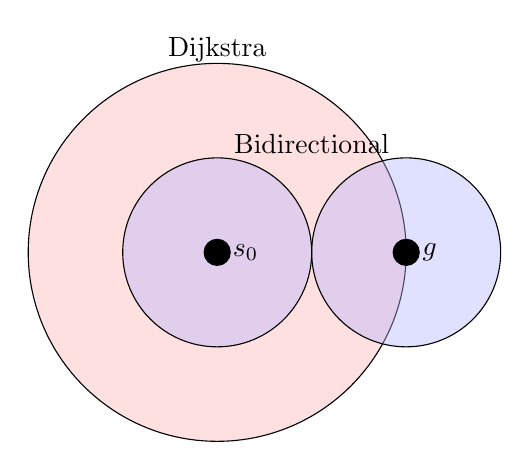
\begin{tikzpicture}[scale=0.6]
    \pgfmathsetmacro{\x}{2}
% forward search
\draw[fill=red!30, fill opacity=0.4] (0, 0) circle (2*\x);

% bidirectional search
\draw[fill=blue!30, fill opacity=0.4] (0, 0) circle (1*\x);
\draw[fill=blue!30, fill opacity=0.4] (2*\x, 0) circle (1*\x);


\node[draw,circle,fill=black] (a) at (0,0) {};
\node (aa) at (0+0.6, 0) {$s_0$};

\node[draw,circle,fill=black] (b) at (2*\x,0) {};
\node (bb) at (2*\x+0.5,0) {$g$};

\node (d) at (0, 2*\x+0.3) {Dijkstra};
\node (a) at (\x, 1*\x+0.3) {Bidirectional};

  \end{tikzpicture}
  }
  \caption{両方向探索}
  \label{fig:bidirectional}
\end{figure}


% \begin{algorithm}
% \caption{両方向幅優先探索 (Bidirectional Breadth-first search)}
% \label{alg:external-brfs}
% 	\Input{非明示的状態空間グラフ $(s, t, Expand, w)$}
% 	\Output{$s$からゴール状態$t$への経路、経路が存在しなければ$\emptyset$}
%         $Open_0 \leftarrow \{s\}$, $Closed_0 \leftarrow \{s\}$, $Open_1 \leftarrow \{t\}$, $Closed_1 \leftarrow \{t\}$\;
%         $\alpha \leftarrow \infty$\;
%         \While {$Open_0 \neq \emptyset$ {\bf and} $Open_1 \neq \emptyset$} {
%           $d \leftarrow 0 \; or \; 1$\;
%           $u \leftarrow \argmin_{u' \in Open_d} f_d(u')$\;
%           $Open_d \leftarrow Open_d \setminus \{u\}$\;
%           $Closed_d \leftarrow Closed_d \cup \{u\}$\;
%           \If {$f_d(u) \geq \alpha$} {
%             \Continue
%           }
%           \If {$u \in Closed_{1-d}$} {
%             $\alpha \leftarrow \min(\alpha, g_d(u) + g_{1-d}(u))$\;
%             $path \leftarrow Path(u)$\;
%           }
% 
%         }
% \end{algorithm}



\section{外部メモリ探索 (External Search)}
\label{sec:external-search}


グラフ探索は重複検出のために今までに展開したノードをすべて保持しなければならない。
よって、保持できるノードの量によって解ける問題が決まってくる。
探索空間があまりに大きすぎると、ノードが多すぎてメモリに乗り切らないということが起きる。

\define{外部メモリ探索}{External Search}{がいぶメモリたんさく}は外部記憶、HDDやSDDを用いることでこの問題を解決する \cite{chiang1995external}。
すなわち、オープンリストとクローズドリストの一部を外部記憶に保持し、必要に応じて参照しメモリに持ってくる、ということをする。
外部メモリ探索のミソは、外部記憶へのアクセス回数をどのように減らすかにある。
表\ref{tbl:latency}は一般的なコンピュータのキャッシュ・メモリ・ハードディスクへのアクセスレイテンシーを比較した表である\footnote{表は\url{(https://gist.github.com/jboner/2841832)}より。}。メモリから1MB{\it 逐次に}読みだすオペレーションは250,000 nanosecかかるが、ハードディスクからの読出しは20,000,000 nanosecもかかる。更にハードディスクにランダムアクセスする場合(Disk seek)は8,000,000 nanosecもかかる。
よって、HDDは工夫して使わなければ実行時間が非常に遅くなってしまう。%\footnote{似たような理由で、HDDを用いないRAMベースの探索を効率化するためにはキャッシュ効率を工夫しなければならない。詳しくは\cite{burns2012implementing}を参照されたい。}。



\begin{table}
\centering
\caption{一般的なハードウェアのアクセス速度。メモリへのアクセス速度に対して外部記憶のアクセスは遅い。加えて、ランダムアクセスはseekの時間がかかるためさらに遅くなる。 }
\label{tbl:latency}
\begin{tabular}{|l|r|}
		   & nano sec \\ \hline
	命令実行 & 1 \\
	L1キャッシュからFetch & 0.5 \\
	分枝予測ミス 		& 5 \\
	L2キャッシュからFetch & 7 \\
	mutexロック・アンロック			& 25 \\
	メインメモリからFetch  	& 100 \\
	SSDから4KBをランダムにRead         & 150,000 \\
	メモリから1MBの連続した領域をRead & 250,000 \\
	ディスクから新しい領域をFetch & 8,000,000 \\
	SSDから1MBの連続した領域をRead		& 1,000,000 \\
	ディスクから1MBの連続した領域をRead 	& 20,000,000 \\
	
\end{tabular}
\end{table}

% \subsection{外部メモリ 幅優先探索 (External BrFS)}
% \label{sec:external-brfs}

一般に外部メモリが効率的であるためには問題に何らかの制約が必要になる。
例えばアルゴリズム\ref{alg:external-brfs}にある\define{外部メモリ幅優先探索}{external breadth-first search}{がいぶメモリはばゆうせんたんさく} (External BrFS)はグラフが無向グラフの時にしかうまくいかない \cite{mehlhorn2002external}。

\begin{figure}
  \centering
  \scalebox{0.75}{
  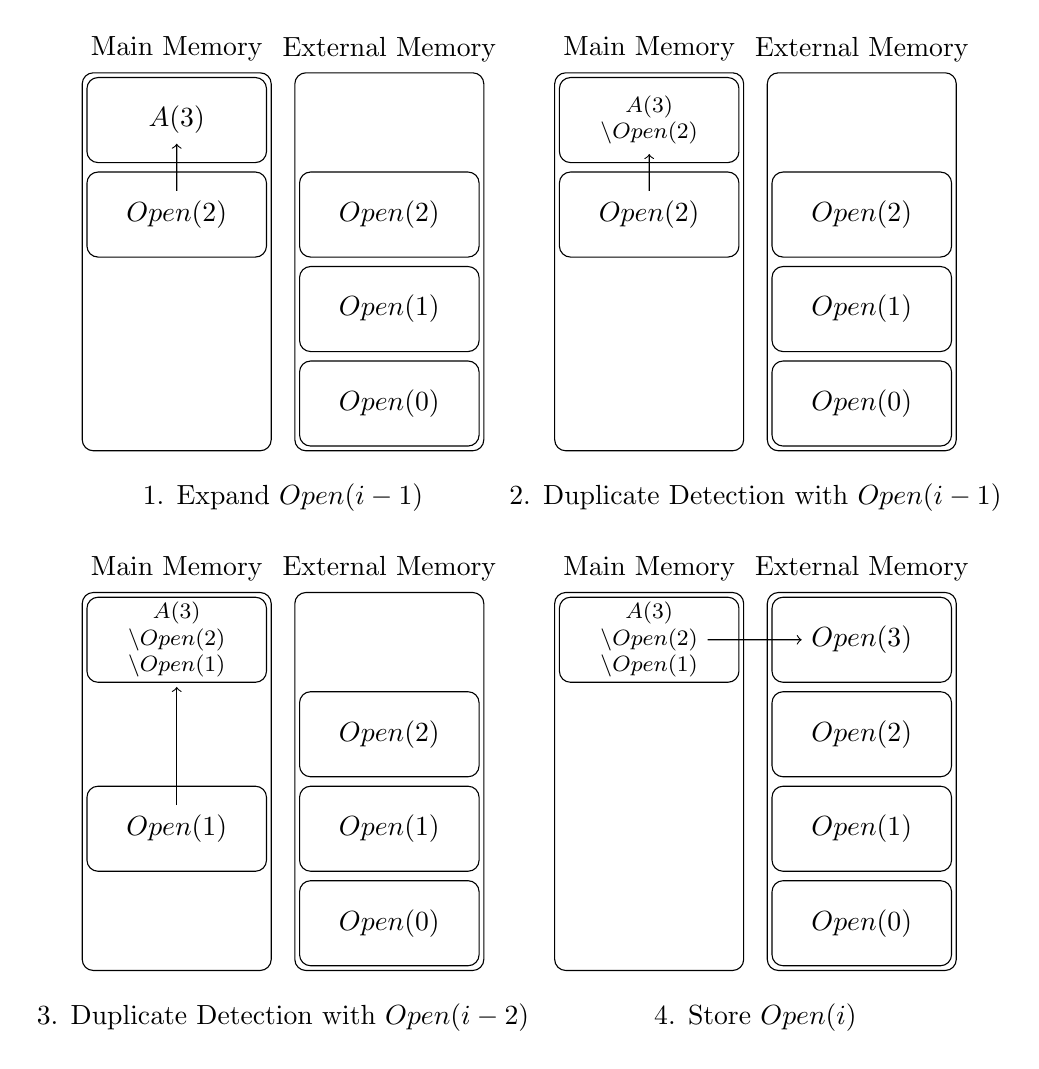
\begin{tikzpicture}[scale=0.6]
    \pgfmathsetmacro{\phi}{0.1}
\pgfmathsetmacro{\sp}{4.5}


%%%%%%%%%%%%%%%%%%%%%%%%
% State 1
%%%%%%%%%%%%%%%%%%%%%%%%

\pgfmathsetmacro{\bs}{0}
\pgfmathsetmacro{\bsy}{0}

% Memory
\draw[rounded corners] (\bs+0,0) rectangle (\bs+4, 8); 

% External disk
\draw[rounded corners] (\bs+\sp,0) rectangle (\bs+\sp+4, 8); 

\foreach \x in {0, 1, 2} {
  \draw[rounded corners] (\bs+\sp+\phi,\x*2+\phi) rectangle (\bs+\sp+4-\phi, \x*2+2-\phi);
  \node (\x) at (\bs+\sp+2,\x*2+1) {$Open(\x)$};
}

\draw[rounded corners] (\bs+\phi,2*2+\phi) rectangle (\bs+4-\phi, 2*2+2-\phi);
\node (mem2) at (\bs+2,2*2+1) {$Open(2)$};

\draw[rounded corners] (\bs+\phi,2*2+2+\phi) rectangle (\bs+4-\phi, 2*2+2+2-\phi);
\node (a2) at (\bs+2,2*2+2+1) {$A(3)$};
\draw[->] (mem2) -- (a2);

\node at ({\bs + (\sp + 4) / 2}, -1) {1. Expand $Open(i-1)$};

\node at ({\bs + 2}, \bsy+8.5) {Main Memory};
\node at ({\bs + \sp + 2}, \bsy+8.5) {External Memory};

%%%%%%%%%%%%%%%%%%%%%%%%
% State 2
%%%%%%%%%%%%%%%%%%%%%%%%

\pgfmathsetmacro{\bs}{10}
\pgfmathsetmacro{\bsy}{0}

% Memory
\draw[rounded corners] (\bs+0,0) rectangle (\bs+4, 8); 

% External disk
\draw[rounded corners] (\bs+\sp,0) rectangle (\bs+\sp+4, 8); 

\foreach \x in {0, 1, 2} {
  \draw[rounded corners] (\bs+\sp+\phi,\x*2+\phi) rectangle (\bs+\sp+4-\phi, \x*2+2-\phi);
  \node (\x) at (\bs+\sp+2,\x*2+1) {$Open(\x)$};
}

\draw[rounded corners] (\bs+\phi,2*2+\phi) rectangle (\bs+4-\phi, 2*2+2-\phi);
\node (mem2) at (\bs+2,2*2+1) {$Open(2)$};

\draw[rounded corners] (\bs+\phi,2*2+2+\phi) rectangle (\bs+4-\phi, 2*2+2+2-\phi);
\node[align=center,font=\footnotesize] (a2) at (\bs+2,2*2+2+1) {$A(3)$\\$\setminus Open(2)$};
\draw[->] (mem2) -- (a2);

\node at ({\bs + (\sp + 4) / 2}, -1) {2. Duplicate Detection with $Open(i-1)$};

\node at ({\bs + 2}, \bsy+8.5) {Main Memory};
\node at ({\bs + \sp + 2}, \bsy+8.5) {External Memory};


%%%%%%%%%%%%%%%%%%%%%%%%
% State 3
%%%%%%%%%%%%%%%%%%%%%%%%

\pgfmathsetmacro{\bs}{0}
\pgfmathsetmacro{\bsy}{-11}

% Memory
\draw[rounded corners] (\bs+0,\bsy+0) rectangle (\bs+4, \bsy+8); 

% External disk
\draw[rounded corners] (\bs+\sp,\bsy+0) rectangle (\bs+\sp+4, \bsy+8); 

\foreach \x in {0, 1, 2} {
  \draw[rounded corners] (\bs+\sp+\phi,\bsy+\x*2+\phi) rectangle (\bs+\sp+4-\phi, \bsy+\x*2+2-\phi);
  \node (\x) at (\bs+\sp+2,\bsy+\x*2+1) {$Open(\x)$};
}

\draw[rounded corners] (\bs+\phi,\bsy+2*1+\phi) rectangle (\bs+4-\phi, \bsy+2*1+2-\phi);
\node (mem1) at (\bs+2,\bsy+2*1+1) {$Open(1)$};

\draw[rounded corners] (\bs+\phi,\bsy+2*2+2+\phi) rectangle (\bs+4-\phi, \bsy+2*2+2+2-\phi);
\node[align=center,font=\footnotesize] (a2) at (\bs+2,\bsy+2*2+2+1) {$A(3)$\\$\setminus Open(2)$\\$\setminus Open(1)$};
\draw[->] (mem1) -- (a2);

\node at ({\bs + (\sp + 4) / 2}, \bsy-1) {3. Duplicate Detection with $Open(i-2)$};

\node at ({\bs + 2}, \bsy+8.5) {Main Memory};
\node at ({\bs + \sp + 2}, \bsy+8.5) {External Memory};



%%%%%%%%%%%%%%%%%%%%%%%%
% State 4
%%%%%%%%%%%%%%%%%%%%%%%%

\pgfmathsetmacro{\bs}{10}
\pgfmathsetmacro{\bsy}{-11}

% Memory
\draw[rounded corners] (\bs+0,\bsy+0) rectangle (\bs+4, \bsy+8); 

% External disk
\draw[rounded corners] (\bs+\sp,\bsy+0) rectangle (\bs+\sp+4, \bsy+8); 

\foreach \x in {0, 1, 2, 3} {
  \draw[rounded corners] (\bs+\sp+\phi,\bsy+\x*2+\phi) rectangle (\bs+\sp+4-\phi, \bsy+\x*2+2-\phi);
  \node (\x) at (\bs+\sp+2,\bsy+\x*2+1) {$Open(\x)$};
}

\draw[rounded corners] (\bs+\phi,\bsy+2*2+2+\phi) rectangle (\bs+4-\phi, \bsy+2*2+2+2-\phi);
\node[align=center,font=\footnotesize] (a2) at (\bs+2,\bsy+2*2+2+1) {$A(3)$\\$\setminus Open(2)$\\$\setminus Open(1)$};

\draw[->] (a2) -- (3);

\node at ({\bs + (\sp + 4) / 2}, \bsy-1) {4. Store $Open(i)$};

\node at ({\bs + 2}, \bsy+8.5) {Main Memory};
\node at ({\bs + \sp + 2}, \bsy+8.5) {External Memory};

  \end{tikzpicture}
  }
  \caption{外部メモリ幅優先探索の操作}
  \label{fig:external-brfs}
\end{figure}

\begin{algorithm}
\caption{外部メモリ幅優先探索 (External Breadth-first search)}
\label{alg:external-brfs}
	\Input{非明示的状態空間グラフ $(\mathcal{E}, u_0, \mathcal{G}, w)$}
	\Output{$u_0$からゴール状態への経路、経路が存在しなければ$\emptyset$}
	$Open(-1) \leftarrow \emptyset$\;
	$Open(0) \leftarrow \{u_0\}$\;
	$i \leftarrow 1$\;
	\While {$Open(i-1) \neq \emptyset$}{
		\If {$\exists (u \in Open(i-1)) \mathcal{G}(u)$} {
			\Return $Path(u)$\;
		}
                
		$R(i) \leftarrow {u | u \in \mathcal{E}(u'), u' \in Open(i-1)}$\;
    \For {each $v \in R(i)$} {
      $parent(v) \leftarrow u$ s.t. $v \in \mathcal{E}(u)$\;
    }
		$Open(i) \leftarrow R(i) \setminus (Open(i-1)\cup Open(i-2))$\;
		$i \leftarrow i + 1$\;
	}
	\Return $\emptyset$\;
\end{algorithm}

外部メモリ幅優先探索は深さ$i$のノードを$Open(i)$に保持する (図\ref{fig:external-brfs})。
$Open(i)$にあるノードを全て展開し、生成されたノードを$R(i)$に保存する。
$R(i)$にあるノードから$Open(i-1), Open(i-2)$と重複したノードを取り除き、残ったノードを$Open(i+1)$に入れる。
このような操作をすることによって、外部メモリ幅優先探索は深さ$i$のノードを展開するときは$Open(i)$のみをメインメモリに保持し、他の展開済みノードはすべて外部メモリに置くことができる。

グラフが無向グラフである場合、状態$u$と同じ状態は深さ$d(u)-2, d(u)-1, d(s)$にしか現れない。
よって深さ$i$のノードの集合$R(i)$は深さ$i-1, i-2$で発見されたノードとだけ重複検出をすれば十分である。
そのためオープンリストの全ノードではなく、$Open(i-1), Open(i-2)$のみを外部メモリから読み込んでくればよい。

もしグラフが有向グラフである場合、$Open(0), Open(1), ..., Open(i-1)$まですべてと重複検出を行う必要があり、その場合外部メモリに何度もアクセスしなければならない。


外部メモリを利用した探索は幅優先に限らず、様々な (整数の) プライオリティ関数に対応してデザインすることができる。
外部メモリA*は外部メモリを用いたA*探索である \cite{edelkamp2004external}。


\section{シンボリック探索 (Symbolic Search)}
\label{sec:symbolic-search}
\define{二分決定グラフ}{Binary Decision Diagram}{にぶんけっていグラフ} (BDD)は二分木によってブーリアンの配列からブーリアンへの関数$\mathbb{B}^n \rightarrow \mathbb{B}$を効率良く表すグラフ構造である \cite{akers1978binary,bryant1992symbolic}。
\define{シンボリック探索}{symbolic search}{シンボリックたんさく}はBDDを使って状態の集合、アクションの集合を表し、BDD同士の演算によって状態の集合を一気に同時に展開していく手法である \cite{edelkamp1998obdds,Edelkamp99deterministicstate}。
A*探索がノードを一つずつ展開していき、一つずつ生成していく手間と比較して非常に効率的に演算が出来るポテンシャルを秘めている。
また、オープン・クローズドリストをBDDで表せられるため、メモリ消費量が少なくなる場合がある。
2014年のInternational Planning CompetitionのSequential Optimal部門(最適解を見つけるパフォーマンスを競う部門)の一位から三位までをシンボリック探索が総なめした \cite{vallati20152014}。


\subsection{特徴表現 (Symbolic Representation)}
\label{sec:symbolic-representation}



\begin{figure}
  \centering
  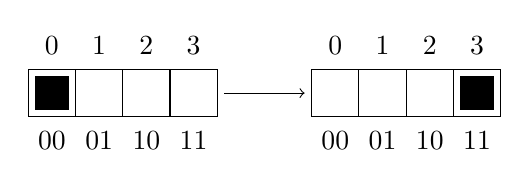
\begin{tikzpicture}[scale=0.6]
    
\pgfmathsetmacro{\phi}{0.15}

\foreach \base in {0, 6} {
  \draw (\base+0,0) grid (\base+4, 1);
  
  \foreach \x in {0, 1, 2, 3} {
    \node at (\base+\x+0.5, 1+0.5) {\x};  
  }

  \node at (\base+0+0.5, -1+0.5) {00};
  \node at (\base+1+0.5, -1+0.5) {01};
  \node at (\base+2+0.5, -1+0.5) {10};
  \node at (\base+3+0.5, -1+0.5) {11};

}

\draw[fill=black] (0+\phi,0+\phi) rectangle (1-\phi,1-\phi);

\draw[fill=black] (6+3+\phi,0+\phi) rectangle (6+4-\phi,1-\phi);

\draw[->] (4+\phi, 0.5) -- (6-\phi, 0.5);

  \end{tikzpicture}
\caption{特徴表現の例}
\label{fig:sliding-token}
\end{figure}


説明のために非常なシンプルなスライディングタイルパズルを考える(図\ref{fig:sliding-token})。
初期状態でタイルは位置0にあり、タイルを右か左に動かすことが出来る。タイルを位置3に動かせばゴールである。
この問題では状態は4通り$(S = \{0,1,2,3\})$しかないが、可能な状態の集合は$2^4$通りある $(2^S = \emptyset, \{0\}, \{1\}, \{2\}, \{3\}, \{0, 1\}, ..., \{0, 1, 2, 3\})$。
オープン・クローズドリストが保持する状態の集合はこのべき集合の要素である ($Open, Closed \in 2^S$)。

\define{特徴表現}{symbolic representation}{とくちょうひょうげん}はこの状態の集合を効率よく表現するための手法である。
状態の集合$O \in 2^S$に対して、ある状態$s$が$O$に含まれているかを返す関数$\phi_{O}: 2^S \rightarrow \{0, 1\}$を\define{特徴関数}{characteristic function}{とくちょうかんすう}と呼ぶ。

\begin{table}
\centering
\caption{特徴関数の例}
\label{tbl:sliding-token}
\begin{tabular}{c|c|c|c}
	状態 & コメント & ブーリアン表現 & 特徴関数 \\ \hline
	0		& 初期状態	& 00				& $\lnot x_0 \lnot x_1$ \\	
	1		& -			& 01				& $\lnot x_0  x_1$ \\	
	2		& -			& 10				& $x_0 \lnot x_1$ \\	
	3		& ゴール状態	& 11				& $x_0 x_1$ \\	
\end{tabular}
\end{table}

$\phi_O$は$O$に含まれる状態を全て明に保持すれば表現することが出来るが、もっと簡潔に表現することもできる。
まず、4通りの状態を2つのブーリアン変数 $s = (x_0, x_1)$で表すと$S = \{00, 01, 10, 11\}$になる。この表現を用いると、例えば$O = \{0\}$とすると、$\phi_{O}(x) = \lnot x_0 \lnot x_1$と表すことが出来る。$O = \{0, 1\}$ならば$\phi_{O}(x) = \lnot x_0$となる。

% 面白いことに、1つの状態のみを含む状態集合$S' = \{0\}$を表す特徴関数よりも要素2つの$S$を表す特徴関数の方が表現がコンパクトになる。
% このように、特徴表現は明示的に列挙するよりも状態の集合をコンパクトに表現出来る場合がある。

アクションによる状態遷移も特徴関数$Trans: S \times S \rightarrow \{0, 1\}$によって定義される。アクション$a \in A$によって状態$x$から$x'$に遷移するならば、$Trans_a(x,x')$は真を返す(かつその時のみ)。
アクション集合$A$による遷移は$Trans(x,x')$によって表現され、$Trans(x,x')$は$Trans_a(x,x')$が真となる$a \in A$が存在する場合に真を返す(かつその時のみ)。

図\ref{fig:sliding-token}の問題で可能なアクションは$(00) \rightarrow (01), (01) \rightarrow (00), (01) \rightarrow (10), (10) \rightarrow (01), (10) \rightarrow (11), (11) \rightarrow (10)$の6つである。これらを表す遷移関数は

\begin{equation}
\begin{split}
	Trans(x,x') &= (\lnot x_0 \lnot x_1 \lnot x'_0 x'_1) \\
		&\lor (\lnot x_0 x_1 \lnot x'_0 \lnot x'_1) \\
		&\lor (\lnot x_0 x_1 x'_0 \lnot x'_1) \\
		&\lor (x_0 \lnot x_1 \lnot x'_0 x'_1) \\
		&\lor (x_0 \lnot x_1 x'_0 x'_1) \\
		&\lor (x_0 x_1 x'_0 \lnot x'_1)
\end{split}
\end{equation}

となる。
アクションのコストがある場合は$Trans(w, x, x')$として表現され、$Trans(x,x')$は$Trans_a(x,x')$が真となる$a \in A$が存在し、かつそのアクションのコストが$w$である場合に真を返す(かつその時のみ)。


\subsection{二分決定グラフ (Binary Decision Diagram)}
\label{sec:binary-decision-diagram}

状態の集合や遷移関数はブーリアンによる特徴関数によって表すことができる。
この特徴関数は\define{二分決定グラフ}{binary decision diagram}{にぶんけっていグラフ} (BDD)というデータ構造によってコンパクトに保持しつつさまざまな集合演算を行うことができる。

\ddef{二分決定グラフ、BDD}{
BDDはループのない有向グラフであり、ノードとエッジはラベルが付いている。単一の根ノードと2つのシンクがあり、シンクのラベルは1と0である。sink以外のノードのラベルは変数$x_i (i \in \{1,...,n\})$であり、エッジのラベルは1か0である。
}

\begin{figure}
  \centering
  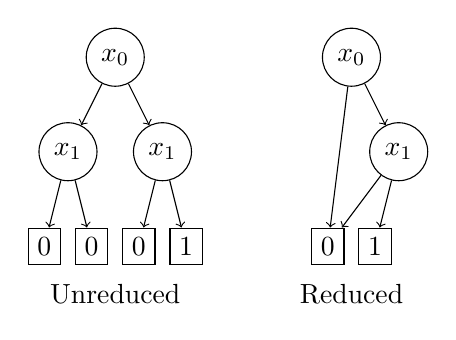
\begin{tikzpicture}[scale=0.6]
    % Unreduced
\node[circle,draw] (00) at (0, 4) {$x_0$};

\node[circle,draw] (10) at (-1, 2) {$x_1$};
\node[circle,draw] (11) at (1, 2) {$x_1$};

\node[rectangle,draw] (20) at (-1-0.5, 0) {$0$};
\node[rectangle,draw] (21) at (-1+0.5, 0) {$0$};
\node[rectangle,draw] (22) at ( 1-0.5, 0) {$0$};
\node[rectangle,draw] (23) at ( 1+0.5, 0) {$1$};

\draw[->] (00) -- (10);
\draw[->] (00) -- (11);

\draw[->] (10) -- (20);
\draw[->] (10) -- (21);
\draw[->] (11) -- (22);
\draw[->] (11) -- (23);

\node at (0, -1) {Unreduced};

% Reduced
\pgfmathsetmacro{\base}{5}
\node[circle,draw] (00) at (\base+0, 4) {$x_0$};

\node[circle,draw] (11) at (\base+1, 2) {$x_1$};

\node[rectangle,draw] (22) at (\base-0.5, 0) {$0$};
\node[rectangle,draw] (23) at (\base+ 0.5, 0) {$1$};

\draw[->] (00) -- (22);
\draw[->] (00) -- (11);

\draw[->] (11) -- (22);
\draw[->] (11) -- (23);

\node at (\base+0, -1) {Reduced};

  \end{tikzpicture}
  \caption{$x_0 x_1$を表す決定木 (左)とBDD (右)}
  \label{fig:bdd}
\end{figure}

BDDは決定木と同様な処理によって入力$x$に対して$\{1, 0\}$を返す。
すなわち、根ノードから始まり、ノードのラベル$x_i$に対して、入力$x$の$x_i$が1であればラベル1が付いたエッジをたどり、0であればラベル0をたどる。これを繰り返し、シンクにたどり着いたらシンクのラベルの値を返す。
決定木と異なりBDDは木ではなく、途中で合流などがあるため、決定木よりも空間効率が良い場合が多い (図\ref{fig:bdd})。
BDDは集合演算によってたくさんの状態に対して同時に展開・重複検知を行い、探索を進めることができる。



\subsection{特徴関数による状態空間の探索}

状態空間の探索は特徴関数の演算によって表現することが出来、その演算はBDDの演算によって実装することが出来る。

ある状態集合$S$に対して、$s \in S$となる$s$の次状態の集合を$S$の{\it image}と呼ぶ。
$S$のimageは以下の特徴関数によって表すことが出来る。

\begin{equation}
	Image_S(x') = \exists x (Trans(x,x') \land \phi_S(x))
\end{equation}

これを使ってグラフ探索アルゴリズムを実装することが出来る。
例えば$Image_{Open}(x')$はオープンリストにあるノードを全て展開して生成されるノードの集合になる。
重複検出にはこの中から$Closed(x)$に入っていないノードを取り出せばよい ($Image_{Open}(x) \land \lnot Closed(x)$)。


imageを繰り返し求めていくことで幅優先木探索は簡単に実装することが出来る。
まず、初期状態$s_0$だけによる集合$S_0 = \{s_0\}$を考える。これに対して$\phi_{S_{i}}$は集合$S_i$を表す特徴関数だとする。これを用いることで次状態集合を次々と求めることが出来る:

\begin{equation}
	\phi_{S_i}(x') = \exists x (\phi_{S_{i-1}}(x) \land Trans(x,x'))
\end{equation}

簡単に言えば、状態$x'$は、もし親状態$x$が$S_{i-1}$に含まれていれば、$S_i$に含まれる。
探索を停止するためには探索した状態にゴール状態が含まれているかをテストしなければならない。
ゴールテストも特徴関数を用いて表すことが出来る。
ゴール状態集合$T$を表す特徴関数を$\phi_T$とすると、$\phi_{S_i}(x') \land \phi_T \neq false$であれば$S_i$はゴール状態を含む。

アルゴリズム\ref{alg:bdd-brfs-tree}はシンボリック幅優先木探索である。
imageの計算とゴールテストによって実装することが出来る。


\begin{algorithm}
\caption{シンボリック幅優先木探索 (Symbolic Breadth-first Tree Search)}
\label{alg:bdd-brfs-tree}
	\Input{非明示的状態空間グラフ $(\mathcal{E}, u_0, \mathcal{G}, w)$}
	\Output{$u_0$からゴール状態への経路、経路が存在しなければ$\emptyset$}
	$S_0 \leftarrow \{u_0\}$\;
	\For {$i \leftarrow 1, 2, ...$} {
		$\phi_{S_i}(x) \leftarrow \exists x (\phi_{S_{i-1}}(x) \land Trans(x,x'))[x'/x]$\;
		\If {$\phi_{S_i}(x) \land \phi_T \neq false$} {
			\Return $Construct(\phi_{S_i} \land \phi_T(x), i)$\;
		}
	}
%	\Return No solution found
\end{algorithm}


$Construct$関数はゴールに至るための経路を計算する関数である。
$\phi_{S_i} \land \phi_T(x)$によってゴール状態、解経路における$i$ステップ目の状態($s_i$)が得られる。次に$Trans(\phi_{S_{i-1}}, s_i)$によって$i-1$ステップ目の状態$s_{i-1}$が得られ、$Trans_a$を見ていくことで$i-1$ステップ目のアクションが得られる。これを繰り返すことによって元の解経路を復元することが出来る。ゴール状態は一つ取り出せば十分であるため、$Construct$の計算時間は大きくはない。

シンボリック幅優先木探索は幅優先探索と同様、解の経路長が最短であることを保証する。


% \subsubsection{シンボリック幅優先グラフ探索}

重複検出を行う場合はクローズドリストに展開済みノードを保存する必要がある。
この展開済みノードも特徴関数及びBDDで表すことが出来る。
アルゴリズム\ref{alg:bdd-brfs}はシンボリック幅優先グラフ探索のコードである。
アルゴリズム\ref{alg:bdd-brfs-tree}と異なり特徴関数$Closed$を用いて重複検出を行っている。

ヒューリスティック関数を用いたシンボリック探索としてはシンボリックA*などがある \cite{edelkamp1998obdds}。
シンボリック幅優先探索では$g$値毎にオープンリストを分けていたがシンボリックA*では$f$値と$h$値のペア毎にオープンリストを分けることで$f$値の小さい状態を優先して探索する。


\begin{algorithm}
\caption{シンボリック幅優先探索 (Symbolic Breadth-first search)}
\label{alg:bdd-brfs}
	\Input{非明示的状態空間グラフ $(\mathcal{E}, u_0, \mathcal{G}, w)$}
	\Output{$u_0$からゴール状態への経路、経路が存在しなければ$\emptyset$}
	$S_0 \leftarrow \{u_0\}$\;
	$Closed \leftarrow \{u_0\}$\;
	\For {$i \leftarrow 1, 2,...$} {
		$Succ(x) \leftarrow \exists x (\phi_{S_{i-1}}(x) \land Trans(x,x'))[x'/x]$\;
		$\phi_{S_i}(x) \leftarrow Succ(x) \land \lnot Closed(x)$\;
		$Closed(x) \leftarrow Closed(x) \lor Succ(x)$\;
		\If {$\phi_{S_i}(x') \land \phi_T \neq false$} {
			\Return $Construct(\phi_{S_i} \land \phi_T(x), i)$\;
		}
	}
%	\Return No solution found
\end{algorithm}

% TODO: BDD-最適コスト探索
% \subsubsection{BDD-最適コスト探索}

% Not for now
%\subsection{Symbolic Tree Search}
%\subsection{Symbolic Blind Search}
%\subsection{Symbolic Heuristic Search}

% \subsection{関連文献}




\section{新奇性に基づく枝刈り (Novelty-based Pruning)}
\label{sec:novelty-based-pruning}

% TODO: 他の枝刈り手法についても紹介する

状態空間を広く探索することは局所最適やデッドエンドに陥らないためには必要である。
より\define{新奇性}{novelty}{しんきせい}のある状態を優先して探索することによって広く状態空間が探索できると考えられる。
状態空間が非常に大きい場合は、よりアグレッシブに、すでに生成された状態と似たような状態を枝刈りしていく方法がある。


%新奇性は似たような状態というのが定義しやすいドメインにおいて有効である。


\subsection{状態の新奇性 (Novelty)}
\label{sec:novelty}

状態に対して新奇性を定義する試みは古くから人工知能研究にある\cite{lehman2008exploiting}。
なので新奇性の定義も様々であるが、本書では\cite{geffner2015}の定義に従い、新奇性を以下のように定義する。

\ddef{新規性、Novelty}{
$m$個の特徴関数の集合$h_1,h_2,....,h_m$に対して新たに生成された状態$s$の新奇性$w(s)$は$n$であるとは、
$n$個の特徴関数によるタプル$\{h_{i_1},h_{i_2},..,h_{i_n}\}$が存在し、
$h_{i_1}(s) = h_{i_1}(s')$, $h_{i_2}(s) = h_{i_2}(s')$,...,$h_{i_n}(s) = h_{i_n}(s')$を満たす生成済みの状態$s'$が存在せず、
かつ、この条件を満たすそれよりも小さいタプルが存在しない。
}

特徴関数は単純に状態変数の値を返す関数を使うことができる \cite{geffner2015, lipovetzky2015a}。
つまり状態$s = \{v_1, v_2,...,v_m\}$に対して特徴関数は$h_i = v_i$とする。
この場合、$w(s) = m$であれば状態変数がすべて同じノードがすでに生成済みであるということなので、$s$は重複したノードである。
このため枝刈りのために新奇性を定義する場合はこれが便利である。

% TODO: もっとわかりやすい例?
% 例えばマルバツゲームの新奇性を考える。
% 特徴関数$h_i$は$i$の位置にあるマーク(空、マル、バツ)を返す。
% 初期状態$s_0$の新奇性は生成済み状態が存在しないので1である。

% \begin{figure}
% TODO: マルバツゲームの図
% \caption{マルバツゲームにおける新奇性の例}
% \end{figure}

\subsection{幅制限探索 (Width-Based Search)}
\label{sec:width-based-search}


\begin{algorithm}
\caption{幅制限探索 (Width-based search)}
\label{alg:width-based-search}
	\Input{非明示的状態空間グラフ $(\mathcal{E}, u_0, \mathcal{G}, w)$、特徴関数 $h_0, h_1,..., h_{m-1}$、幅$i$}
	\Output{$u_0$からゴール状態への経路、経路が存在しなければ$\emptyset$}
	$Open \leftarrow \{u_0\}$, $Closed \leftarrow \emptyset$\;
	\While{$Open \neq \emptyset$} {
                $u \leftarrow \argmin_{u' \in Open} f(u')$ \;
		$Open \leftarrow Open \setminus \{u\} $\;
		\If {$\mathcal{G}(u)$} {
			\Return $Path(u)$\;
		}
		\For {each $v \in \mathcal{E}(u)$} {
                  $H(v) \leftarrow \{j | j \in \{0, 1, ..., m-1\}, h_j(v) = 1\}$\;
                  $H \leftarrow \{j | j \in \{0, 1, ..., m-1\}, h_j(v) \in Closed\}$\;
                  \If{$|H \setminus Closed| \geq i$} {
                    $Open \leftarrow Open \cup \{v\}$\;
                    $parent(v) \leftarrow u$\;
                  }
                  \For {each $h \in H(v) \setminus Closed$} {
                    $Closed \leftarrow Closed \cup \{h\}$\;
                  }
		}
 	}
	\Return $\emptyset$\;
\end{algorithm}

\define{幅制限探索}{width-based search}{はばせいげんたんさく}は状態の新奇性に基づいてノードを枝刈りする手法である \cite{lipovetzkyg12}。
新奇性によってノードを枝刈りするので、解が存在しても発見される保証はない (完全性を満たさない)。

IW($i$)は新奇性が$i$よりも大きい状態を枝刈りする探索である。
新奇性に基づく枝刈りには2つのメリットがある。
一つは状態空間が著しく小さくなる。
もう一つは幅を制限することで生成済みノードをクローズドリストにすべて保存する必要がなくなる。
その代わり保存しなければならない情報は、生成済みの特徴のタプルのうち大きさが$i$以下のものの集合である。
これがないと新奇性を計算することができない。
IWにおけるクローズドリストは過去に真であったことのある特徴の集合である。
状態$s$において真である特徴の集合を$H$としたとき、$H$に存在し$Closed$に存在しない特徴の数が$i$以上かどうかを確認し、$i$以上であればそのノードを生成する。そうでなければ枝刈りを行う。

幅$i$を大きくするほど発見できる解のクオリティが上がりやすいが、一方探索空間は$i$に対して指数的に大きくなっていく。
このトレードオフを調整しやすくするために新奇性の定義域を有理数に拡張した幅制限探索が提案されている\cite{geffner2015}。


\subsection{反復幅制限探索 (Iterative Width Search)}
\label{sec:iterative-width-search}

\define{反復幅制限探索}{iterative width search}{はんぷくはばせいげんたんさく}は幅制限探索を幅を大きくしながら解を発見するまで繰り返すアルゴリズムである \cite{lipovetzkyg12}。
IW($i$)は幅$i$が大きくなるほど解のクオリティが良くなるが、より大きな状態空間を探索することになる。
反復幅制限探索は小さい幅からはじめ、解が見つからない・良い解でなければ幅を大きくして再度探索を行う手法である。
いずれ幅の大きさが特徴の数と同じまでになるので、反復幅制限探索は解があればいずれ必ず発見する。

\begin{algorithm}
\caption{反復幅制限探索 (Iterative Width Search)}
$i \leftarrow 1$\;
$P \leftarrow \emptyset$\;
	\While {$P = \emptyset$} {
		$P \leftarrow IW(i)$\;
		$i \leftarrow i + 1$\;
	}
	\Return $path$
\end{algorithm}

\begin{comment}

\subsection{Best-First Width Search (最良優先幅制限探索)}
\label{sec:width-based-heuristic-search}

\cite{geffner2015}


\subsection{Novelty Heuristics (新奇性に基づくヒューリスティック)}
\label{sec:novelty-heuristics}

ここまでの議論では新奇性を枝刈りのために使った。
しかしノードを捨ててしまう枝刈りは解が存在する問題でも解を発見できなくなってしまうという問題がある。
新奇性を使ってノードを完全に捨ててしまうのではなく、新奇性に基づいてノードを展開する優先度を決めるというアプローチをとることができる \cite{geffner2015}。つまり新奇性をヒューリスティックに使うということである。
この方法ではノードは完全に捨てられることはないので解を捨ててしまう可能性はなくなる。

ここで注意しなければならないのは新奇性は生成済みノード集合に依存する値である。
つまり新奇性に基づくヒューリスティック関数は状態$s$の関数ではなく、状態とクローズドリストの関数となる。つまり、同じ状態のノードでもヒューリスティック値が異なる場合がある。

\end{comment}

% \subsection{関連文献}
% Best-First Width Search (最良優先幅制限探索) \cite{geffner2015}
% Novelty Heuristics (新奇性に基づくヒューリスティック) \cite{geffner2015}


\section{並列探索 (Parallel Search)}
\label{sec:parallel-search}

近年コンピュータ一台当たりのコア数は増加を続けており、コンピュータクラスタにも比較的容易にアクセスが出来るようになった。Amazon Web Serviceのようなクラウドの計算資源も普及し、将来的には並列化が当然になると考えられる。
並列化の成功例は枚挙にいとまないが、近年のディープラーニングはまさに効率的な並列計算アーキテクチャによって得られたブレイクスルーであるといえる。
%残念ながら、探索アルゴリズムの並列化は比較的難しいと考えられる。
%一般に並列アルゴリズムの効率は逐次実行部分と並列実行可能部分に分割される
%グラフ探索アルゴリズムを並列化するメリットの一つはもちろん実行速度の高速化である。
グラフ探索アルゴリズムの並列化に考えなければならないオーバーヘッドは様々であり、それらの重要性は問題、インスタンス、マシン、さまざまな状況に依存する。% 加えてハードウェアは刻々と変化を続けており、数年後にどのような環境がメジャーとなるのかはなかなか想像をすることが出来ないだろう。
% 本書ではCPUを用いた分散メモリ並列アルゴリズムとGPU一台を用いた並列アルゴリズムについて説明する。
CPU並列ではハッシュによってノードを各プロセスにアサインし、各プロセスはアサインされたノードのみを担当して探索を行うというフレームワークが有効である。
より詳細な議論は\cite{fukunaga2017survey}を参照されたい。

\subsection{並列化オーバーヘッド (Parallel Overheads)}
\label{sec:parallel-overheads}

理想的には$n$プロセスで並列化したら$n$倍速くなってほしい。
逐次アルゴリズムと比較して、プロセス数倍の高速化が得られることを\define{完全線形高速化}{perfect linear speedup}{かんぜんせんけいこうそくか}と呼ぶ。
しかしながら、殆どの場合完全線形高速化は得られない。
それは並列化にさいして様々なオーバーヘッドがかかるからである。
\cite{jinnai2017work}の記法に従うと、並列化オーバーヘッドは主に以下の3つに分けられる。

\ddef{通信オーバーヘッド、communication overhead}{
  プロセス間で情報交換を行うことにかかる時間を\define{通信オーバーヘッド}{communication overhead}{つうしんオーバーヘッド} (CO)と呼ぶ。
}

通信する情報は様々なものが考えられるが、オーバーヘッドとなるものはノードの生成回数に比例した回数通信を必要とするものである。
すなわち、ノードの生成回数$n$に対して$log(n)$回しか通信を行わない場合、その通信によるオーバーヘッドは無視出来るだろう。
ここではノードの生成回数に対するメッセージ送信の割合をCOと定義する:
\begin{equation}
	CO := \frac{\text{他プロセスへ送信されたメッセージの数}}{\text{生成されたノードの数}}.
\end{equation}
例えば、ハッシュなどによってプロセス間でノードの送受信を行いロードバランスを行う手法 (e.g. 後述するHDA*)の場合、通信するメッセージは主にノードである。この場合:

\begin{equation}
	CO := \frac{\text{他プロセスへ送信されたノードの数}}{\text{生成されたノードの数}}.
\end{equation}
となる。
COは通信にかかるディレイだけでなく、メッセージキューなどのデータ構造の操作も行わなければならないので、特にノードの展開速度が速いドメインにおいて重要なオーバーヘッドになる。一般に、プロセス数が多いほどCOは大きくなる。
%If nodes are assigned randomly to the threads, CO will be proportional to $1-\frac{1}{\#thread}$. 

\ddef{探索オーバーヘッド、Search Overhead}{
  並列化によって余分に増えた展開ノード数の割合を探索オーバーヘッドと呼ぶ。
}

一般に並列探索は逐次探索より多くのノードを展開することになる。
このとき、余分に展開したノードは逐次と比較して増えた仕事量だと言える。
本書では以下のように探索オーバーヘッドを定義する:

\begin{equation}
  SO := \frac{\text{並列探索で展開されるノード数}}{\text{逐次探索で展開されるノード数}} - 1.
\end{equation}

SOは\define{ロードバランス}{load balance}{ロードバランス} (LB)が悪い場合に生じることが多い。

\begin{equation}
LB := \frac{\text{各プロセスに割り当てられたノード数の最大値}}{\text{各プロセスに割り当てられたノード数の平均}}.
\end{equation}

ロードバランスが悪いと、ノードが集中しているスレッドがボトルネックとなり、他のスレッドはノードがなくなるか、あるいはより$f$値の大きい(有望でない)ノードを展開することになり、探索オーバーヘッドになる。

探索オーバーヘッドは実行時間だけでなく、空間オーバーヘッドでもある。ムダに探索をした分だけ、消費するメモリ量も多くなる。分散メモリ環境においてもコア当りのRAM量は大きくなるわけではないので、探索オーバーヘッドによるメモリ消費は問題となる。

\ddef{同期オーバーヘッド、Coordination Overhead} {
  他のスレッドの処理をアイドル状態で待たなければならない時間の割合を\define{同期オーバーヘッド}{coordination overhead}{どうきオーバーヘッド}と呼ぶ。
}

アルゴリズム自体が同期を必要としないものだとしても、メモリバスのコンテンションによって同期オーバーヘッドが生じることがある\cite{burnslrz10,kishimotofb13}.


これらのオーバーヘッドは独立ではなく、トレードオフの関係にある。
多くの場合、通信・同期オーバーヘッドと探索オーバーヘッドがトレードオフの関係にあたる。


\subsection{並列A* (Parallel A*)}

\define{並列A*}{parallel A*}{へいれつエースター} (PA*)はA*探索のシンプルな並列化である \cite{iranis86}。PA*は一つのオープンリスト・クローズドリストを全てのプロセスで共有してアクセスする。オープンリスト・クローズドリストには複数のプロセスが同時にアクセスできないようにロックがかけられる。
PA*の問題点はデータ構造を一つに集中させているため、分散メモリ環境の場合はアクセスに大きな通信オーバーヘッドが生じることである。
共有メモリ環境の場合でも、それぞれのプロセスは他のプロセスがデータ構造にアクセスしている間にはアクセスできないため、同期オーバーヘッドが生じる。この同期オーバーヘッドはプロセスの数が増えるほど問題になる。ロックフリーのデータ構造を使ってもこのオーバーヘッドは解消されない \cite{burnslrz10}。

\subsection{ハッシュ分配A* (Hash Distributed A*)}
\label{sec:hash-distributed-astar}

PA*の問題点はすべてのプロセスが共有された一つのデータ構造へアクセスしなければならない点である。このような手法を\define{集中型手法}{centralized approach}{しゅうちゅうがたしゅほう}と呼ぶ。
共有データ構造へのアクセスは計算のボトルネックとなり、スケーラビリティの限界点になってしまう。
そのため、A*の並列化には各プロセスが自分のオープンリスト・クローズドリストを持ち、アクセスを分散させる\define{分散型手法}{decentralized approach}{ぶんさんがたしゅほう}が有力である。
分散型手法はデータ構造へのアクセスが分散するため同期オーバーヘッドを解消される。一方、各プロセスがアクセスするデータ構造が異なるため、各プロセスの仕事量を均等に分配しずらいという\define{ロードバランシング}{load balancing}{ロードバランシング}の問題が生じる。各プロセスに対してどのようにして仕事を均等に分配するかが問題になる。

\define{ハッシュ分配A*}{Hash Distributed A*}{ハッシュぶんぱいエースター} (HDA*) \cite{kishimotofb13}はstate-of-the-artの並列A*探索アルゴリズムである。
HDA*の各プロセスはそれぞれローカルなオープンリスト、クローズドリストを保持する。ローカルとは、データ構造を保持するプロセスが独占してアクセスを行い、他のプロセスからはアクセスが不可能であるという意味である。
グローバルなハッシュ関数によって全ての状態は一意に定まる担当のプロセスが定められる。
各プロセス$T$の動作は以下を繰り返す (アルゴリズム\ref{alg:hdastar}):

\begin{enumerate}
	\item 
		プロセス$T$はメッセージキューを確認し、ノードが届いているかを確認する。届いているノードのうち重複でないものをオープンリストに加える(A*同様、クローズドリストに同じ状態が存在しないか、クローズドリストにある同じ状態のノードよりも$f$値が小さい場合に重複でない)。
	\item 
		オープンリストにあるノードのうち最もプライオリティ($f$値)の高いノードを展開する。生成されたそれぞれのノード$n$についてハッシュ値$H(n)$を計算し、ハッシュ値$H(n)$を担当するプロセスに非同期的に送信される。
\end{enumerate}


\begin{algorithm}
  \caption{Hash Distributed A*}
  \Input{非明示的状態空間グラフ $(\mathcal{E}, u_0, \mathcal{G}, w)$、ヒューリスティック関数$h$、ハッシュ関数 $H$}
  \Output{$u_0$からゴール状態への経路、経路が存在しなければ$\emptyset$}
  $Closed_p \leftarrow \emptyset$, $Open_p \leftarrow \emptyset$, $\mathit{Buffer}_p \leftarrow \emptyset$ for each thread $p$\;
  $Open_{H(u_0)} \leftarrow \{u_0\}$, $g(u_0) \leftarrow 0$\;
  $goal \leftarrow \emptyset$, $c' \leftarrow \infty$\;

  \For {each process $p$} {
  \While {{\bf not} $TerminateDetection()$} {
    \For {each $(v, g_v, p_v) \in \mathit{Buffer}_p$} {
      \If{$v \notin Closed$ {\bf or} $g_v < g(v)$} {
        $Open \leftarrow Open \cup \{v\}$\;
	$g(v) \leftarrow g_v$\;
        $parent(v) \leftarrow p_vv$\;
      }
      \If{$v \notin Closed$} {
        $Closed \leftarrow Closed \cup \{v\}$\;
      }
    }
    $\mathit{Buffer}_p \leftarrow \emptyset$\;
    \While {$Open_p \neq \emptyset$ {\bf and} $min_{s \in Open_p} f(s) < c'$} {
      $u \leftarrow \argmin_{u' \in Open} f(u')$ \;
      $Open \leftarrow Open \setminus \{u\} $\;

      \If {$\mathcal{G}(u)$ {\bf and} $g(u) < c'$} {
        $goal \leftarrow u$\;
        $c' \leftarrow g(u)$\;        
      }

      \For {each $v \in \mathcal{E}(u)$} {
        $g_v \leftarrow g(u) + w(u, v)$\;
        $\mathit{Buffer}_{H(v)} \leftarrow \mathit{Buffer}_{H(v)} \cup \{(v, g_v, u)\}$\;
      }
    }
  }
  \Return $Path(goal)$\;
  }
  \label{alg:hdastar}
\end{algorithm}

HDA*の重要な特徴は2つある。
まず、HDA*は非同期通信を行うため、同期オーバーヘッドが非常に小さい。
各プロセスがそれぞれローカルにオープン・クローズドリストを保持するため、これらのデータ構造へのアクセスにロックを必要としない。
次に、HDA*は手法が非常にシンプルであり、ハッシュ関数$Hash: S \rightarrow {1..P}$を必要とするだけである ($P$はプロセス数)。
%並列アルゴリズムにおいて手法がシンプルであることは非常に有用である。
しかしながらハッシュ関数は通信オーバーヘッドとロードバランスの両方を決定する為、その選択はパフォーマンスに非常に大きな影響を与える。

HDA*が提案された論文\cite{kishimotofb13}ではZobrist hashing \cite{zobrist:70}がハッシュ関数として用いられていた。
状態$s = (x_1,x_2,...,x_n)$に対してZobrist hashingのハッシュ値$Z(s)$は以下のように計算される:

\begin{equation}
\label{eq:zobrist}
 	Z(s) := R_{0}[x_{0}]\; xor\; R_{1}[x_{1}]\; xor\; \cdots\; xor\; R_{n}[x_{n}]%
\end{equation}

Zobrist hashingは初めにランダムテーブル$R$を初期化する\ref{alg:init-zobrist-hashing}。
これを用いてハッシュ値を計算する。

\begin{algorithm}
	\caption{Zobrist Hashing}
	\Input{$s = (x_0, x_1,...,x_n)$}
	$hash \leftarrow 0$\;
	\For {each $x_i \in s$} {
		$hash \leftarrow hash \; xor \; R[x_i]$\;
	}
	\Return $hash$\;
	\label{alg:zobrist-hashing}
\end{algorithm}

\begin{algorithm}
	\caption{Zobrist Hashingの初期化}
	\Input{$V = (dom(x_0),dom(x_1),...)$}
	\For {each $x_i$} {
		\For {each $t \in dom(x_i)$ } {
			$R_i[t] \leftarrow random()$\;
		}
	}
	\Return $R = (R_1, R_2,...,R_n)$
	\label{alg:init-zobrist-hashing}
\end{algorithm}

Zobrist hashingを使うメリットは2つある。
一つは計算が非常に速いことである、XOR命令はCPUの演算で最も速いものの一つである。かつ、状態の差分を参照することでハッシュ値を計算することが出来るので、アクション適用によって値が変化した変数の$R[x]$のみ参照すれば良い。
もうひとつは、状態が非常にバランスよく分配され、ロードバランスが良いことである。
一方、この手法の問題点は通信オーバーヘッドが大きくなってしまうことにある。
この問題を解決するためにState abstractionという手法が提案された\cite{burnslrz10}。
State abstractionは状態$s = (x_1,x_2,...,x_n)$に対して簡約化状態 (abstract state) $s' = (x_1',x_2',...,x_m'), \; where \; m < n, x_i' = x_j (1 \leq j \leq n)$. % TODO: clean up this.
State abstractionは簡約化状態からハッシュ値への関数の定義はされておらず、単純なlinear congrugent hashingが用いられていた。そのため、ロードバランスが悪かった。

Abstract Zobrist hashing (AZH)はZobrist hashingとAbstractionの良い点を組み合わせた手法である\cite{jinnai2016structured}。AZHはfeatureからabstract featureへのマッピングを行い、abstract featureをZobrist hashingへの入力とするという手法である:

\begin{equation}
\label{eq:abstract-zobrist}
 	Z(s) := R_{0}[A_0(x_{0})]\; xor\; R_{1}[A_1(x_{1})]\; xor\; \cdots\; xor\; R_{n}[A_n(x_{n})]%
\end{equation}

ここで関数$A$はfeatureからabstract featureへのマッピングであり、$R$はabstract featureに対して定義されている。
% Abstract featureを自動的に生成する手法は複数提案されており、最もシンプルなものはGreedy abstract feature generation \cite{jinnai2016automated}である。

HDA*のための分配関数の自動生成方法は\cite{jinnai2017work}にまとめられている。


\section{Python実装}

分枝限定法の実装は再帰による。再帰による深さ優先探索のコードとほぼ同様である。

\inputpython{python/branch_and_bound.py}{1}{46}

反復深化深さ優先探索は、再帰による深さ優先探索のコードを変更するだけで実装できる。

\inputpython{python/depth_first_iterative_deepening.py}{1}{52}

反復深化A* (IDA*)はこのコードを使えばプライオリティ関数を変えるだけで実装できる。

\inputpython{python/iterative_deepening_astar.py}{1}{4}

並列探索の実装は手間がかかる。
特に計算機クラスターなどの分散メモリ環境で動くコードを実装するためにはMPIライブラリなどを使い、message passingを行う必要がある。
ここでは1台のコンピュータで実行される共有メモリ環境で動くコードを実装する。
プロセスではなくスレッドを使って並列化を行う。

\inputpython{python/parallel_graph_search.py}{1}{164}

この実装は早くなっただろうか?おそらくこの実装で実行した場合、並列化の恩恵を受けることはほとんどないだろう。
並列化の恩恵を受けるためには、より複雑な問題を解くか、あるいはより洗練されたmessage passingを行う必要がある。



\section{まとめ}

ヒューリスティック探索の手法は数多く提案されており、それぞれ様々な長所・短所がある。
時間・空間制限がありA*探索ではうまくいかない条件であっても、別のヒューリスティック探索手法であれば解決できるかもしれない。
すべての状況で有効な手法は存在しないため、状況に応じて適切な手法を選択する必要がある。

これらの手法はA*探索と比較してやや複雑なため、実装するのに苦労するかもしれない。
可能であれば、その手法を実装して試す前に事前に「その手法で本当に目の前の問題を解決できるのか?」を見積もることが出来るとよいだろう。

\section{練習問題}

\begin{enumerate}
	\item あなたはグリッド経路探索問題を解こうとしている。あなたの目的は経路を見つけることであり、その経路の長さは重要ではない。このとき分子限定法を用いることは適切か?
	
	\item (難問) 直感的には両方向探索は有効に思えるかもしれないが、実はほとんどの場合単方向探索の性能を超えることが難しい。何故だろうか?

	\item 反復深化A*探索とA*の秒間のノードの展開速度を比較してみよう。どちらの方が速いだろうか?また、どのような問題に対してどちらの方が適しているだろうか?

	\item 今あなたはある状態空間問題を解こうとしている。経験的に、A*探索を使った時解の深さが$d$程度である場合まで解けていることが分かっている。それ以上解が深い場合はメモリが足りず解くことが出来ないようである。
	このとき、外部メモリA*探索を使うことで、どのくらいの深さまで解くことができるか見積もることはできるだろうか?ただし、その問題の分枝度は4であり、外部メモリはおよそ内部メモリの1000倍程度であるとする。

	\item さらに解が深い問題を解くためにはどのようなアルゴリズムを使うと良いだろうか?このとき実行時間に制限はないものと仮定する。
		
	\item どのような特徴を持った問題であれば並列化によって解の発見を高速化しやすいだろうか?
\end{enumerate}

\section{関連文献}

両方向探索で正方向ではゴール状態までのコストの推定、逆方向では初期状態までのコストの推定を用いたヒューリスティック探索をFront-to-End戦略と呼ぶ \cite{pohl1971bi}。Front-to-Front戦略は反対方向のオープンリストに入っている状態への距離の推定を用いたアルゴリズムである \cite{sint1977improved}。
Front-to-Front戦略はコストの推定がより正確である代わりに各オープンリストに入っている状態のペアすべてに対してヒューリスティック値を計算し、それを更新し続けなければならない。
Perimiter searchはこの問題を解決するため、探索の方向を一度だけ変える手法である\cite{dillenburg1994perimeter,manzini1995bida}。最初は逆方向探索である深さまで探索をしてからあとは正方向で探索を行う。

\cite{zhou2004structured}は状態空間をいくつかの部分空間に分割し、その分割内でそれぞれオープン・クローズドリストを持つというStructured Duplicate Detectionを用いた外部メモリ探索を提案した。
Solid state drive (SSD)はHDDと比べて高速なだけでなく、得意なアクセスパターンが異なる。SSDの特徴を利用した外部メモリ探索アルゴリズムも提案されている \cite{lin2018revisiting}。

現在提案されているシンボリック探索はほとんどBDDを用いたものである。
BDD以外のデータ構造、例えばZero-surpressed Decision Diagram \cite{minato1993zero}などをヒューリスティック探索に使う例は著者の知る限りない。

% TODO: Novelty-based pruning

\cite{kumar1988parallel}は並列深さ優先探索のさまざまな実装を比較した。
ハッシュ関数によって状態をプロセスに振り分けるアイディアはParallel Retracting A* (PRA*)からである\cite{evett1995massively}。PRA*はプロセス間の同期処理が行っていたのに対して、Transposition Table Driven Work Distribution (TDS) \cite{romein1999transposition}は同期処理を行わないことによって性能を改善した。

執筆時現在、GPUやFPGAなどを用いたアルゴリズムはあまり例がない。
GPU-Parallel A*はオープンリストをいくつものキューに分けて並列化した\cite{zhou2015massively}。
探索にGPUを用いる場合の一番の問題はGPUのメモリが非常に小さいことである。
そのためA*ではなくIDA*の並列化の研究もおこなわれている\cite{horie2017block}。
GPUとCPUの両方を使った探索アルゴリズムも提案されている\cite{sulewskiek11}。

% 
% 
% 一方、執筆時現在、GPUを用いたアルゴリズムはあまり研究が進んでいない。原因としては、既存のCPUを用いた探索アルゴリズムにはない様々な難しさがあるだろう。
% たとえば、GPUはスレッド当りのメモリ量が非常に少ない。A*探索はメモリが大きなボトルネックであり、メモリ量が少ないとそのまま解ける問題の大きさが制限されてしまう。この問題を解決する方法は提示されていない。
% もうひとつの難しさは、GPUは複数のスレッドが同じ命令を実行するSingle instruction multiple thread (SIMT)という計算モデルであることである。そのため、既知の有力なヒューリスティック関数をGPU環境において効率的に実装する方法が自明ではない。
% パターンデータベースなどのシンプルな命令によるヒューリスティックも考えることが出来るが、このようなヒューリスティックは今度はメモリを沢山消費するという問題点がある。
% 効率的なGPU並列化アルゴリズムの開発は大きな成果が期待されるブルーオーシャンであるといえる\footnote{個人の感想である}。
% もしCPU/GPUを利用した効率的なグラフ探索アルゴリズムが開発出来れば、非常に大きなインパクトになるかもしれない。


%  
% \section{モンテカルロ木探索 (Monte Carlo Tree Search)}
% \label{sec:mcts}
% 
% モンテカルロ木探索 (Monte Carlo Tree Search, MCTS)は非常に多様な問題で応用されている手法である。
% その長所はたくさんある。
% まず、MCTSは状態空間が非決定論的でも扱える。不完全情報でも扱える。
% 2人プレイヤーゲームなどにも使える。特に碁で使われている。Alpha Goでも使われた。
% 
% MCTSのエージェントは木データ構造を保持する。
% 木の根は初期状態(2人プレイヤーゲームなどでは現在の盤面を初期状態とする)である。
% MCTSは初期状態から木を辿り、木に新しいノードを追加する、というイテレーションを繰り返す。
% 一つのイテレーションは4つの処理のループからなる。
% 
% \begin{enumerate}
% \item Select a next node following a tree policy
% \item Add a new node to the tree
% \item Simulate following a default policy
% \item Back propagate
% \end{enumerate}
% 
% 
% 
% \begin{algorithm}
% \caption{Monte Carlo Planning(state)}
% \label{alg:mcts}
% 	\While {True} {
%     	search(state, 0)
%     }
%     \Return bestAction(state, 0)
% \end{algorithm}
% 
% \begin{algorithm}
% \caption{search(state, depth)}
% \label{alg:mcts-iter}
% 	\If {Terminal(state)} {
%     	\Return 0
%     }
%     \If {Leaf(state, d)} {
%     	\Return Evaluate(state)
%     }
%     action $\leftarrow$ selectAction(state, depth)\;
%     (nextstate, reward) $\leftarrow$ simulateAction(state, action)\;
%     q $\leftarrow$ reward + $\gamma$ search(nextstate, depth + 1)\;
%     UpdateValue(state, action, q, depth)
% \end{algorithm}
% 
% \subsection{UCT (UCB1 Applied to Tree)}
% \label{sec:uct}
% 
% MCTSのtree policyの選択は状態空間をどのように探索するかに大きな影響を与える。
% 最も広く使われているtree policyはUCB1による \cite{UCT 2006,survey論文}。
% 
% \begin{equation}
% 	UCB1(s, s') = \bar{X_{s'}} + 2 C_p \sqrt{\frac{2 \ln n(s)}{\ln n(s')}}
% \end{equation}
% 
% where $\bar{X_{s'}}$ is the average reward from visiting $s'$, $n(s), n(s')$ is a number of visits to state $s$, $s'$, respectively.
% UCB1を使うMCTSはUpper bound applied to tree (UCT)と呼ばれる。
% 
% \section{その他の派生アルゴリズム}
% ここで紹介した以外にもヒューリスティック探索の派生アルゴリズムはたくさんある。
% 
% \define{再帰的最良優先探索}{Recursive best-first search} (RBFS)はIDA*の拡張である \cite{RBFS}。
% RBFSはノードを最良優先の順で展開し、ヒューリスティック値をバックアップする。
% 余ったメモリを使ってノードの展開数を抑える拡張が提案されている (Memory-aware RBFS) \cite{MRBFS}。
% 
% %Depth-first iterative deepening
% Partial Expansion A* \cite{}。多重整列問題。
% 
% K-Best First Search
% 
% K-ビームサーチ
% Partial A*
% Partial IDA*
% MA*
% Frontier Search
% 
% 
% ポートフォリオ戦略
% どれか一つのアルゴリズムに絞らなくてもよい
% いろいろ試してみるのが有効なことが多い

